
\chapter{Exercise 8}
\label{cha:ugeopgave-8}

The purpose of this exercise is to understand and implement shadow mapping. This includes a deep understanding of the different coordinate spaces in the pipeline as well as mapping between these coordinate spaces.

\section{Part 1}

Implementations of the methods \emph{getLightProjection()} and \emph{getLightView()} are below.

\begin{lstlisting}
mat4 getLightProjection() {
	float d=length(teapotPosition-lightPosition);
	float theta = asin(teapotBoundingRadius/d)
                    *RADIAN_TO_DEGREE;
	mat4 perspective = Perspective(2*theta, 1, 0.1, 400.);
	return perspective;
}
\end{lstlisting}
\smallskip
\begin{lstlisting}
	return LookAt(lightPosition, 
                teapotPosition, vec3(0,1,0));

\end{lstlisting}



\section{Part 2}

After following the description given in exercise document, I render the teapot on shadow map. A screenshot of resulting scene can be seen in Figure \ref{fig:8-2}

\begin{figure}[hp]
\centering
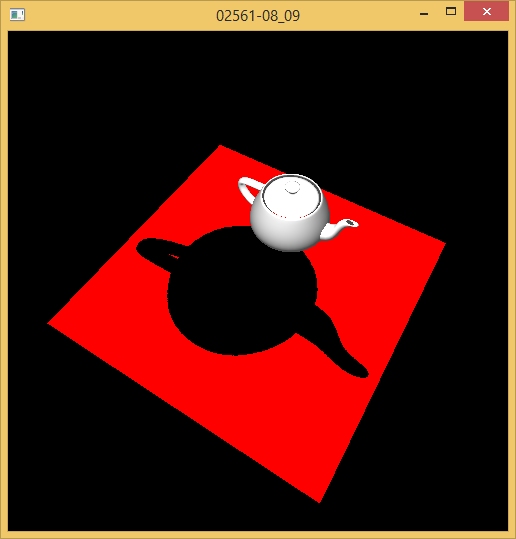
\includegraphics[width=8cm]{../Screenshots/ex-8/2.png}
\caption{Rendering teapot on shadow map}
\label{fig:8-2}
\end{figure}

\section{Part 3}

I compute normalized device coordinated. I transform and map this coordinates to shadow map coordinates, ranging from $(0,0)$ to $(1,1)$. I make the transformation by multiplying normalized device coordinates with bias matrix. The visualisation of shadowUV instead of texture lookup in shaders results in the scene presented in Figure \ref{fig:8-3}.

\begin{figure}[hp]
\centering
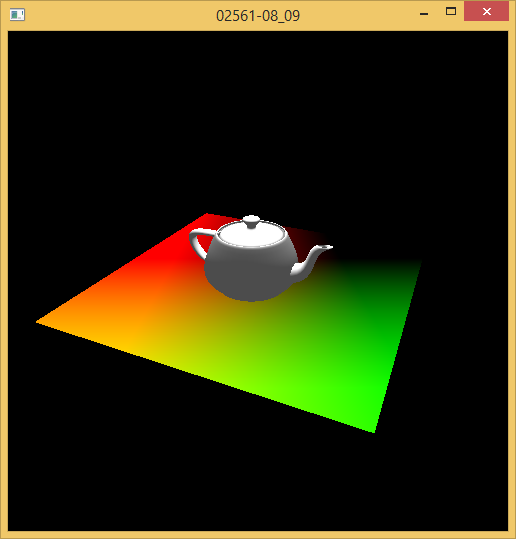
\includegraphics[width=8cm]{../Screenshots/ex-8/3.png}
\caption{Visualisation of shadowUV on plane}
\label{fig:8-3}
\end{figure}

\section{Part 4}

I use these code fragment in fragment shader to decide whether a fragment is in shadow or not: \\

\begin{lstlisting}
vec4 blue= texture(texture1, vTextureCoordinate);
vec4 colors=texture(texture2, shadowUV);
if(colors.x<1)
	fragColor=colors;
else
	fragColor = blue;
\end{lstlisting}


The resulting scene can be seen in Figure \ref{fig:8-4}.

\begin{figure}[hp]
\centering
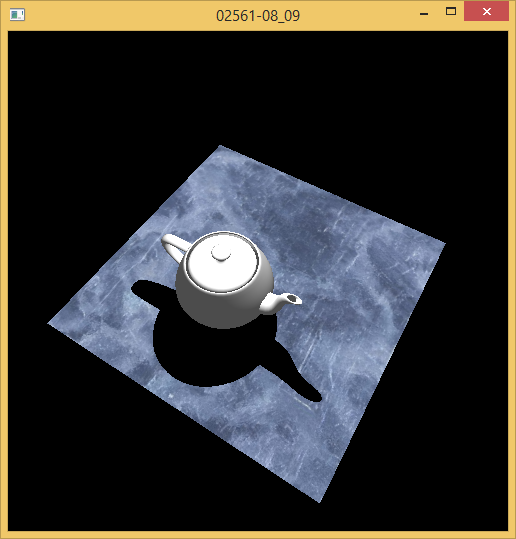
\includegraphics[width=8cm]{../Screenshots/ex-8/4.png}
\caption{The final shadow map texture}
\label{fig:8-4}
\end{figure}

%%% Local Variables:
%%% mode: latex
%%% TeX-master: "report_main"
%%% End: 